 
\section{The Big Picture}

The architecture of this platform can be easily put in a picture.

\begin{center}
  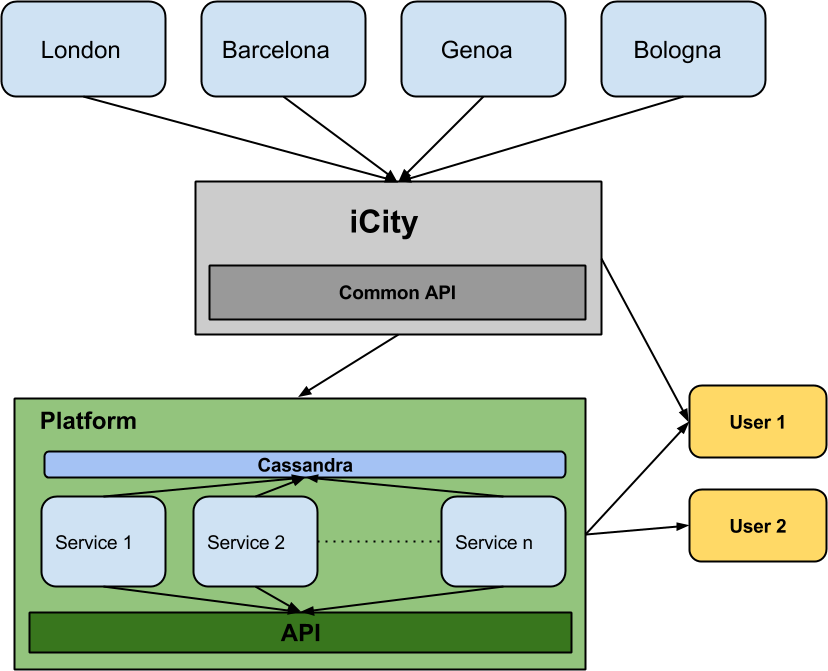
\includegraphics[scale=0.8]{overview/images/big.png}
\end{center}

Let us enumerate what we can see in the picture above:

\begin{enumerate}
  \item The cities of London, Barcelona, Genoa and Bologna are {\bf producers}.
This list of cities will expand over time. Users are {\bf consumers}. They can
consume from either the iCity API or from the API from my platgform or from
both.
  \item The {\bf iCity} platform offers a common API that integrates all the
cities. It gets the data from the different cities and allows the access of
this data to any user registered in the iCity platform.
  \item My {\bf platform} acts as a user of the iCity API and users can access
the processed data.
  \item This platform is formed by {\bf several} services. These services
consume the data from the iCity platform in order to produce the requested
information.
  \item All the services from this platform are available through an {\bf API}.
  \item All the services are part of a {\bf Storm} topology.
  \item All the services share the {\bf state} of the platform, and it is stored
in a Cassandra instance.
\end{enumerate}

